% Following previos finding, this chapter will research and implement a Recurrent Neural Network using voltage, current, temperature and known state of a battery charge to predict and feed-forward the outputted result.
% It meant to use methodology constructed from the previos chapter:
% \begin{itemize}
%     \item Use sigle cell data over entire temperature range for a single profile, use FUDS for better performance capture.
%     \item Train a model with recomended modifications.
%     \item Verefy model against another cell with the same profile.
%     \item Validate the performance against other two profiles, DST and US06.
% \end{itemize}

%
%
%There has been several attempts to determine the most effective strategy for model training.
%Both LSTM and Gradient Recurrent Unit has shown to be effective, and there is no obvios difference on the impact between speed and outputted accuracy.
The previous chapter has analysed and discussed multiple implementations of RNN models to determine the State of Charge from sensory data like Voltage, Current and Temperature.
The research results have concluded that sensory data in one driving behaviour effectively predicts that specific driving behaviour but is poot at extrapolating to others.
\textcolor{red}{Thus, the battery state became a matter of not the battery itself but the way it has been used.
Besides, the SoC can fail under-voltage drop under some scenarios, although not as significant and only at certain rate conditions.}
A potential solution to the problem is integrating SoC as one of the input features to a NN model.
The limitation here is to be able to get the State of Charge in real-time.
There are two approaches to this, use Charge estimation from other means, CC or three feature-based NN methods, or using the Feed-Forward method to propagate the output value of the charge as an input into the next prediction.

%
%
To address some of the limitations identified in Chapter 3, it will require implementing a new 4-feature based model.
In this chapter, the Long short-term memory model will be developed, with a history of 8.5 minutes usage, to predict the current State of Charge and propagate the result further into the next prediction.
Furthermore, a novel method of the training loop model will be proposed to eliminate the possibility of accumulating error and the charge value.
It utilises the Autoregressive technique to introduce an adaptive and robust solution to training with some training output inaccuracy over time.
It meant to force the model to consider the potential of having variations in State of Charge history and yet not fail the prediction output further.

%
%
% The rest of this paper is organised as follows: a methodology for an RNN model discussed in Section 2.
% The details of how auto-regression has been utilised in Section 3.
% Subsections 4.1 and 4.2 separates points of model validation and process of parameters estimation.
% Finally, section 5 concludes the research along with outlining several observations, which may require separate consideration.
% Most were isolated to closed scenarios with provided data or from battery cycling machine.
% The most promessing approches to improve a model and make it more universal is to increase complexity. While some introduced deeper layer newtwork, others added additional mechanisms to already used.
\begin{landscape}
    \begin{figure}[ht]
        \centering
        % 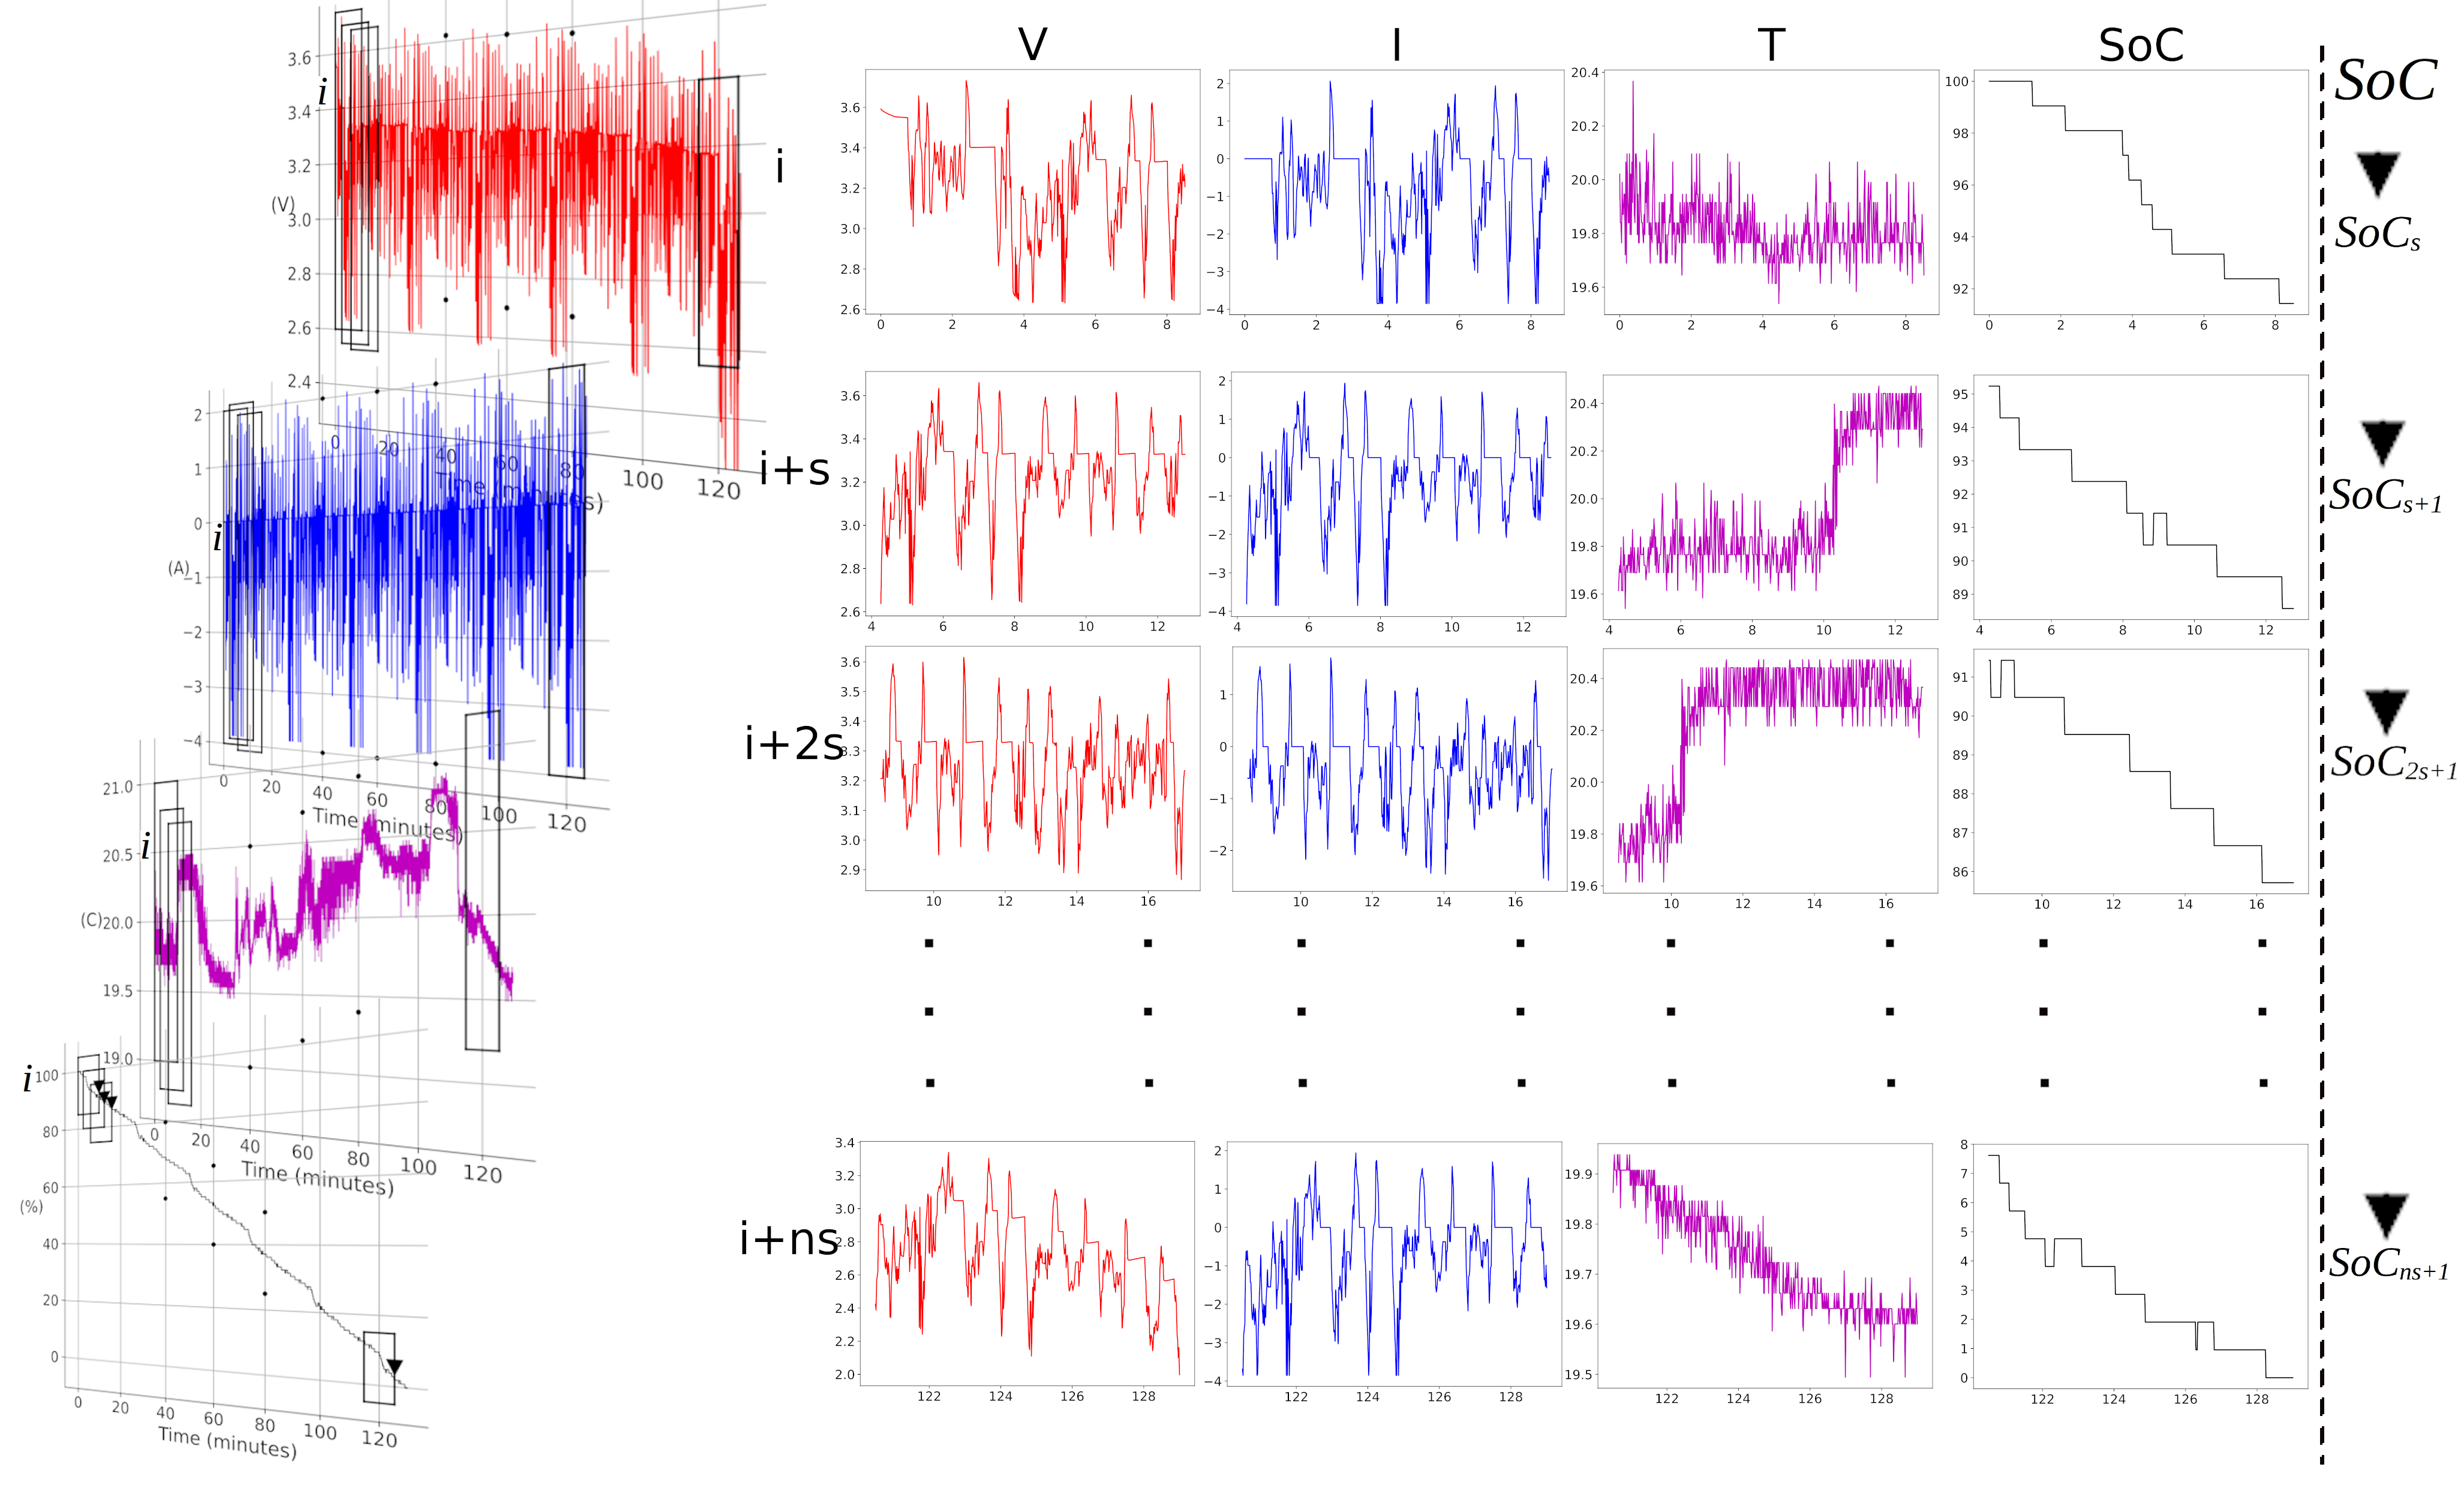
\includegraphics[width=0.9\linewidth]{II_Body/images/Windowing3D-1.jpg}
        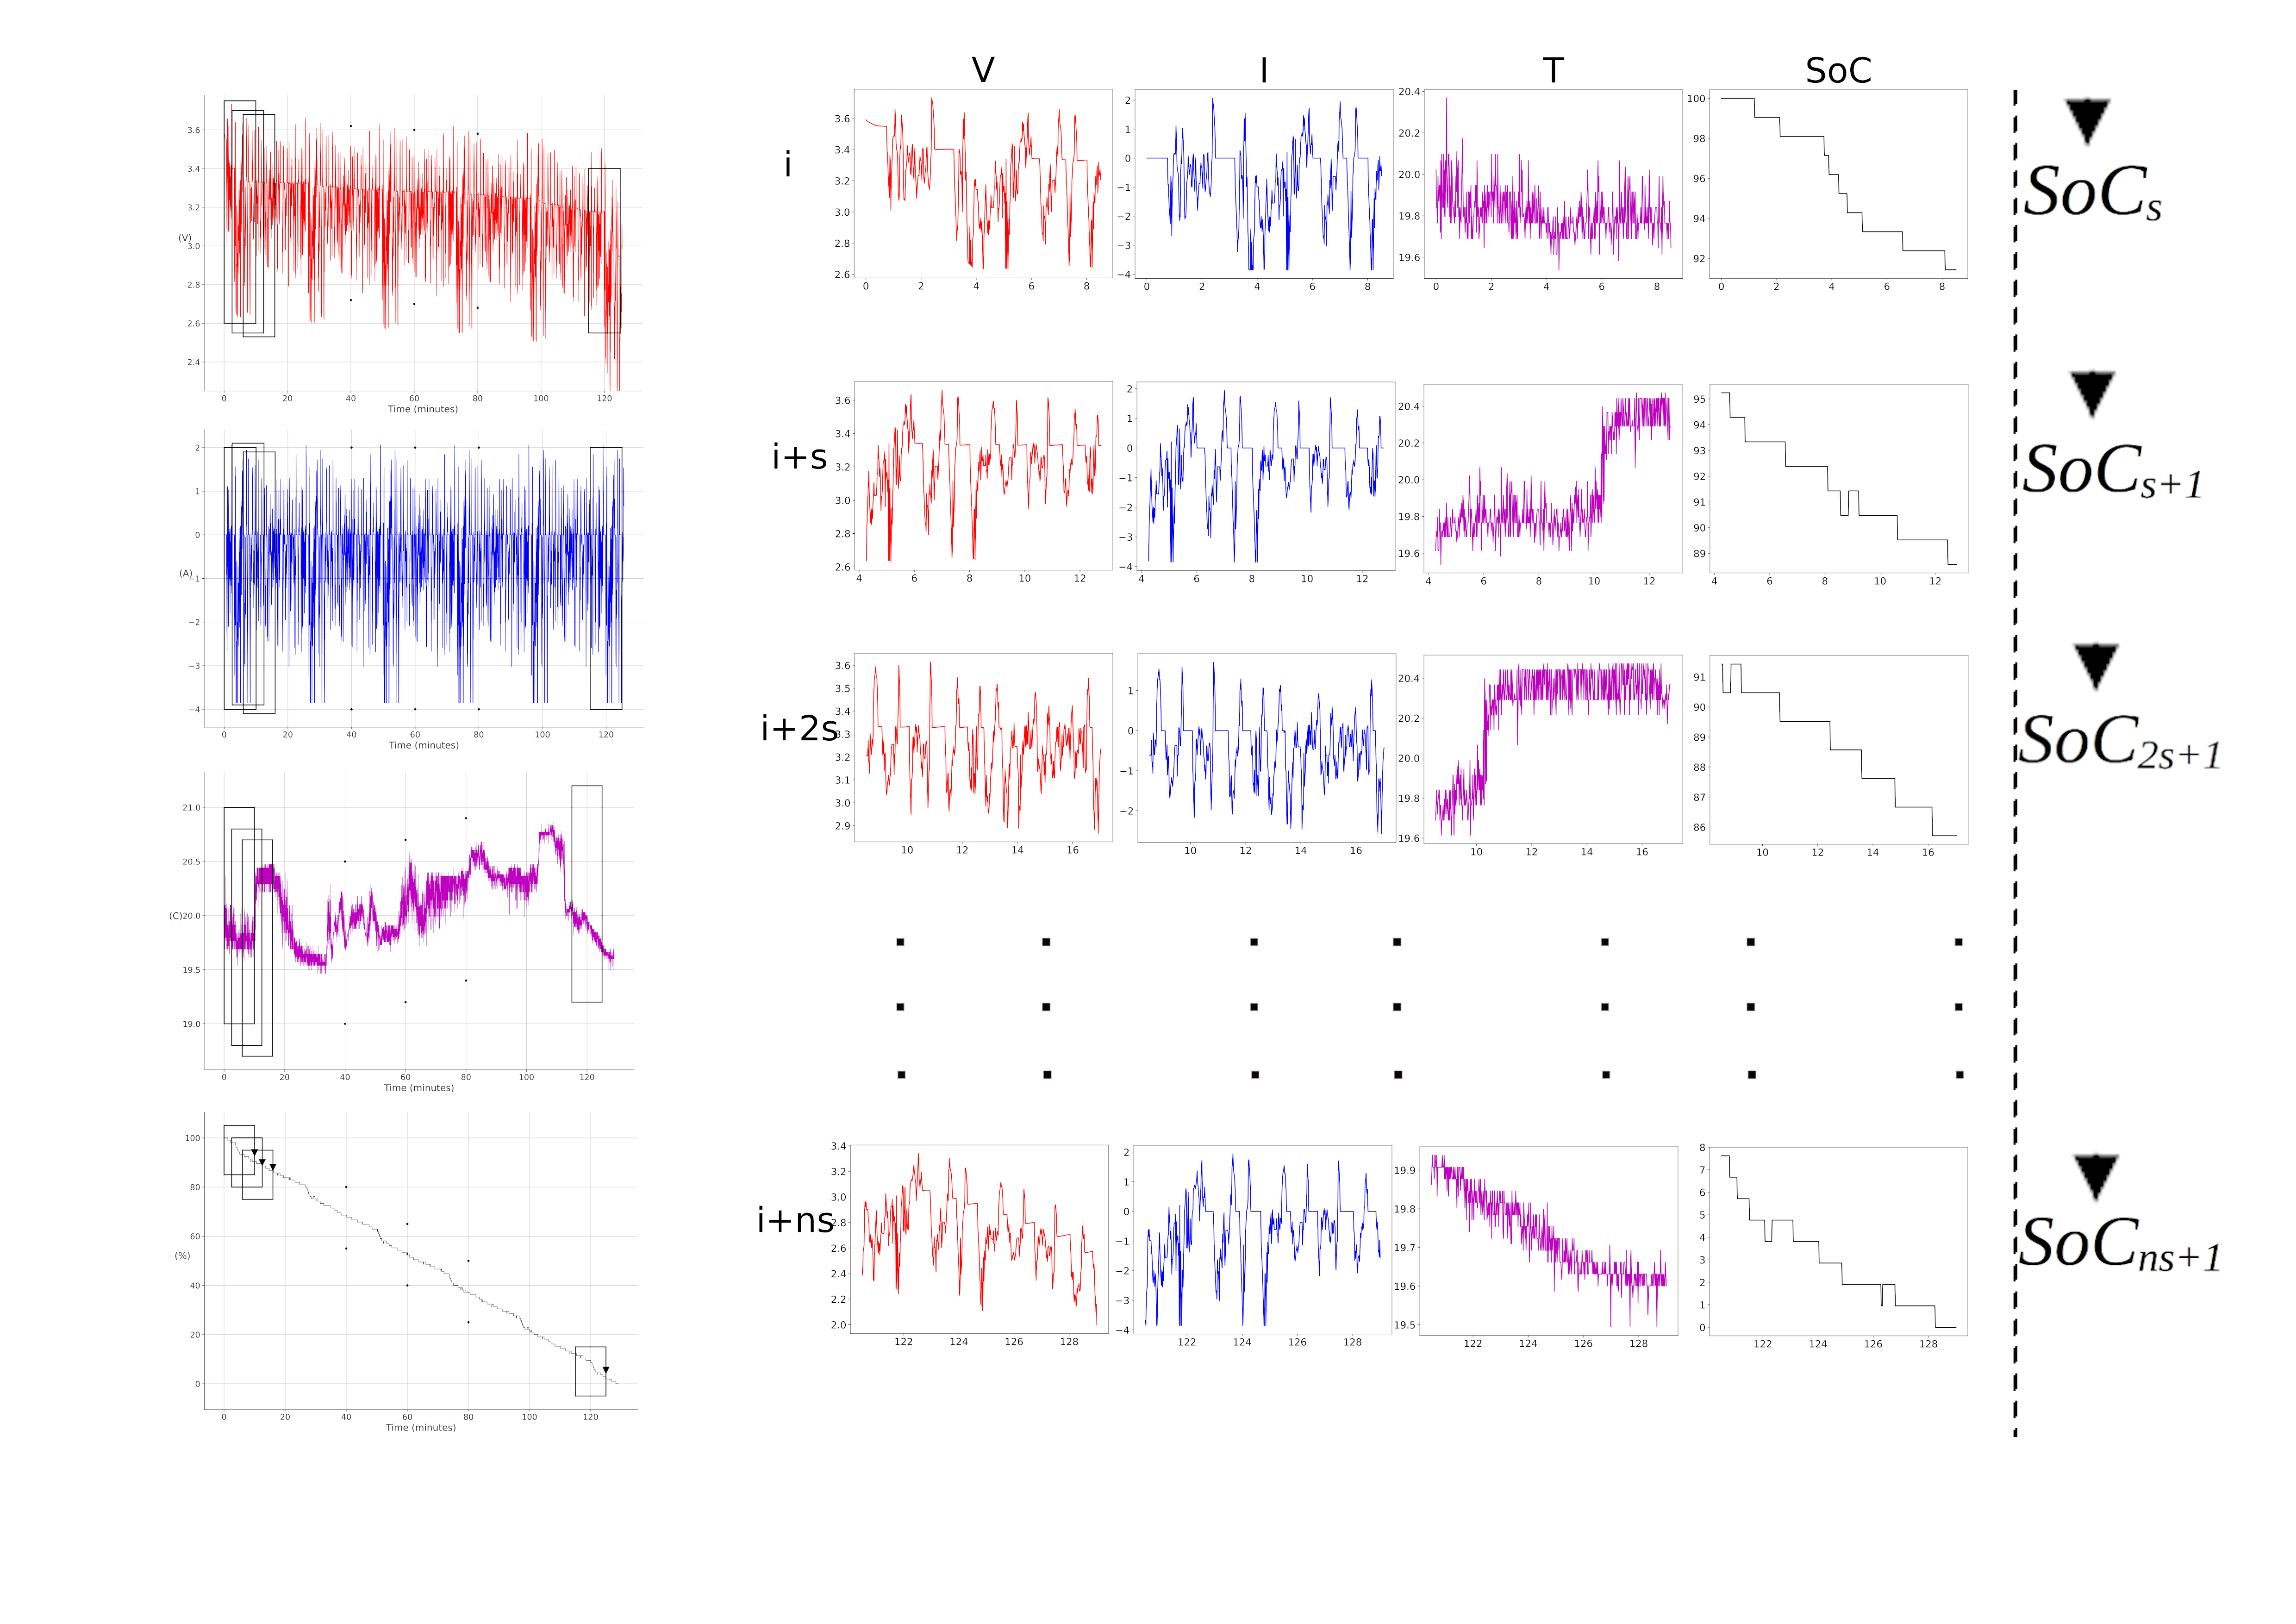
\includegraphics[width=0.9\linewidth]{II_Body/images/Windowing4f-A3.jpg}
        \caption{Data Windowing scheme. For visualisation purposes, the $s$-step has been used as 5 minutes, which is different from actual implementation. Initial index $i$ was kept as a value close to the beginning of the data, around zero.}
        \label{fig:Windowing}
    \end{figure}
\end{landscape}